\section{EVALUATION}
\label{chap:evaluation}

This section presents the quantitative evaluation of the proposed
\textbf{PredCLOCK} system. The performance is analyzed in two phases:
first, a comparative analysis against standard and theoretical
baselines to establish overall efficacy, and second, a deep dive into
model configuration and parameter tuning to understand the impact of
loss functions on cache behavior.

\subsection{Overall Performance Comparison}
\label{sec:overall_performance}

To evaluate the effectiveness of the proposed solution, PredCLOCK was
benchmarked against three references: Standard CLOCK (Baseline),
Optimal Zipf Promotion (Heuristic Oracle), and Offline CLOCK
(Theoretical Upper Bound). The experiments were conducted across four
cache sizes: 1\%, 10\%, 20\%, and 40\% of the total unique object footprint.

Table~\ref{tab:comparison_all} summarizes the performance trade-offs.
Negative values in "Delta Miss Ratio" indicate improvement (reduction
in misses), while positive values indicate regression.

\begin{table}[t]
  \centering
  \small
  \caption{Performance Comparison: PredCLOCK vs. Baselines}
  \label{tab:comparison_all}
  \begin{tabular}{l l r r}
    \toprule
    \textbf{Size} & \textbf{Method} & \textbf{Delta Miss} &
    \textbf{Prom. Red.} \\
    \midrule
    1\% & \textbf{PredCLOCK} & -0.05\% & 10\% \\
    & Optimal Zipf & -0.20\% & 10\% \\
    & Offline CLOCK & -0.35\% & 40\% \\
    \addlinespace
    10\% & \textbf{PredCLOCK} & -0.10\% & 10\% \\
    & Optimal Zipf & -0.90\% & 13\% \\
    & Offline CLOCK & -1.80\% & 43\% \\
    \addlinespace
    20\% & \textbf{PredCLOCK} & -0.20\% & 10\% \\
    & Optimal Zipf & -1.67\% & 15\% \\
    & Offline CLOCK & -3.50\% & 43\% \\
    \addlinespace
    40\% & \textbf{PredCLOCK} & +0.15\% & 8\% \\
    & Optimal Zipf & -3.30\% & 17\% \\
    & Offline CLOCK & -8.00\% & 43\% \\
    \bottomrule
  \end{tabular}
\end{table}

\subsubsection{Analysis of Cache Efficiency}
The results highlight a clear non-linear performance pattern. In
environments with high memory pressure (cache sizes 1\%--20\%),
\textbf{PredCLOCK} provides a "double benefit": a modest reduction in
Miss Ratio (-0.05\% to -0.20\%) and a consistent reduction in memory
writes (promotions). This confirms that the model successfully
identifies "one-hit wonders" (wasted objects) during scan phases,
preventing them from polluting the cache \cite{Tang1976Cache, Breslau1999Web}.

However, at the 40\% cache size, a performance regression (+0.15\%)
is observed. This indicates that the static decision threshold
becomes \textit{over-selective} when cache space is abundant. The
model continues to reject marginal objects that could have been
stored without penalty, leading to valid data being discarded.

\subsubsection{Analysis of Write Efficiency vs. Theoretical Bounds}
A key contribution of PredCLOCK is the reduction of memory write
operations. Across all tested scenarios, the system reduces the
promotion rate by approximately \textbf{8--10\%}. While this is
significant for extending the endurance of flash-based storage (SSDs)
\cite{Sun2022NCache, Wang2018Efficient}, it falls significantly short
of the \textbf{43\%} reduction achieved by \textit{Offline CLOCK}.

This gap highlights the limitations of local-feature prediction
compared to the global future knowledge possessed by the
\textit{Offline CLOCK} oracle \cite{chen2025lazy}. PredCLOCK remains
conservative, prioritizing cache safety (Hit Ratio) over maximum
write reduction.

\subsection{Model Parameter Tuning and Configuration}
\label{sec:model_tuning}

The performance of PredCLOCK is highly sensitive to the handling of
class imbalance. In Zipfian workloads ($\alpha \approx 1.0$), the
ratio of "wasted" objects (accessed once) to "reused" objects is
approximately 80:20. Without intervention, machine learning models
tend to bias towards the majority class. We evaluated two distinct
model configurations: Conservative (Weighted) and Aggressive (Unweighted).

\begin{figure*}[t]
  \centering
  \begin{subfigure}{0.48\textwidth}
    \centering
    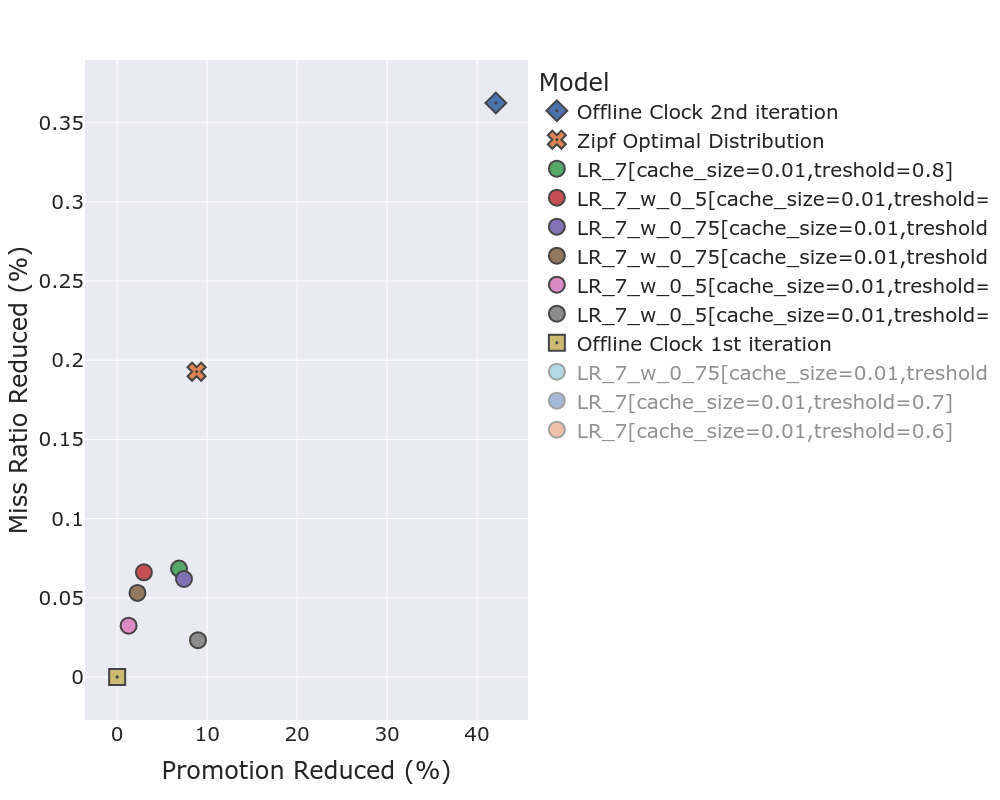
\includegraphics[width=\linewidth]{gambar/hasil/cache_size_0_01.png}
    \caption{1\% Cache Size}
    \label{fig:res_1pct}
  \end{subfigure}
  \begin{subfigure}{0.48\textwidth}
    \centering
    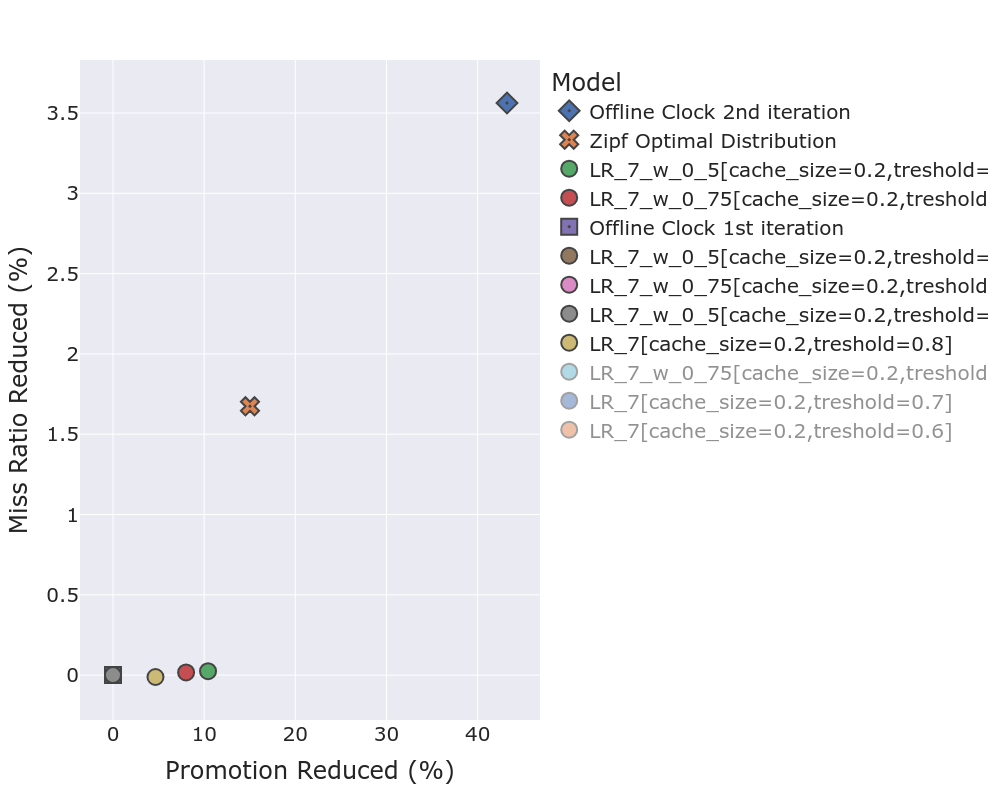
\includegraphics[width=\linewidth]{gambar/hasil/cache_size_0_2.png}
    \caption{20\% Cache Size}
    \label{fig:res_20pct}
  \end{subfigure}
  \caption{Conservative Model performance across cache sizes.
    Note the slight improvement at 1\% and the regression at 40\% due
  to over-selection.}
  \label{fig:conservative_grid}
\end{figure*}

\subsubsection{Configuration A: Conservative Model (Weighted Loss)}
This variant was trained using a custom weighted loss function (ratio
2:1), explicitly penalizing False Positives (incorrectly evicting a
popular object) more heavily than False Negatives. A high decision
threshold (0.8) was applied to ensure objects are only rejected when
the model is highly confident.

The results, visualized in Figures \ref{fig:res_1pct} through
\ref{fig:res_20pct}, show that this configuration successfully mimics
the safety of the standard CLOCK algorithm.

\begin{enumerate}
  \item \textbf{Performance stability:} The Miss Ratio closely tracks
    the baseline, avoiding service degradation.
  \item \textbf{Controlled Efficiency:} The promotion reduction is
    capped at roughly 10\%, representing a safe trade-off between
    hardware endurance and cache hit rates.
\end{enumerate}

\begin{figure*}[t]
  \centering
  \begin{subfigure}{0.48\textwidth}
    \centering
    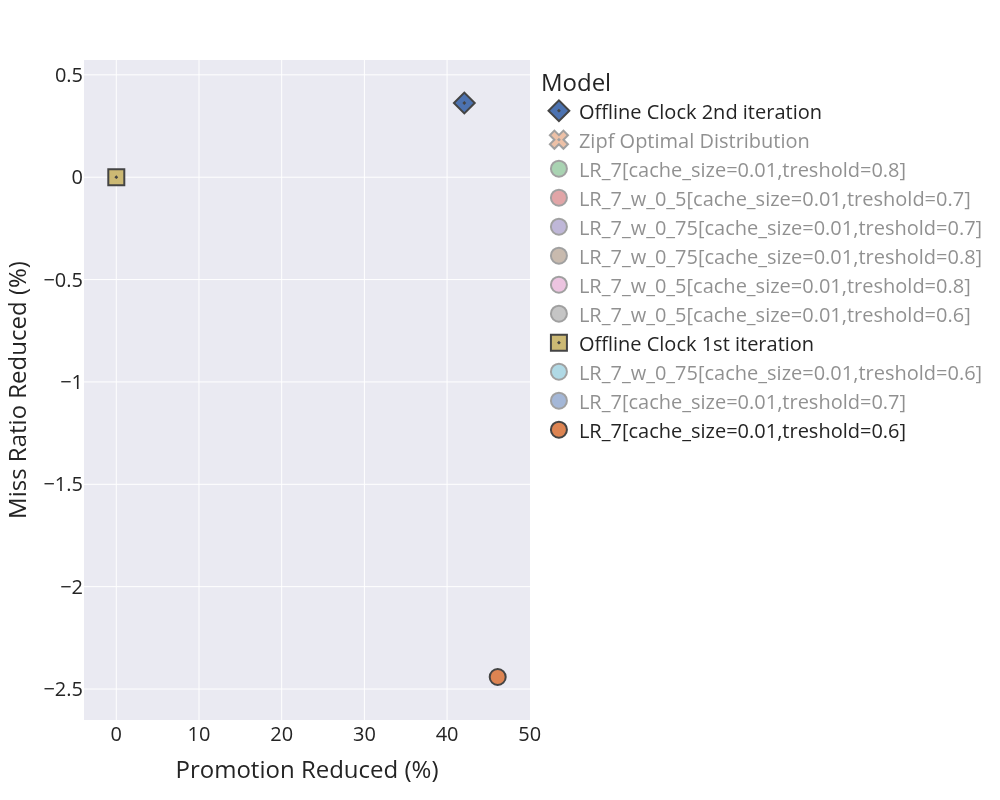
\includegraphics[width=\linewidth]{gambar/hasil/aggressive_0_01.png}
    \caption{1\% Cache Size}
    \label{fig:agg_1pct}
  \end{subfigure}
  \hfill
  \begin{subfigure}{0.48\textwidth}
    \centering
    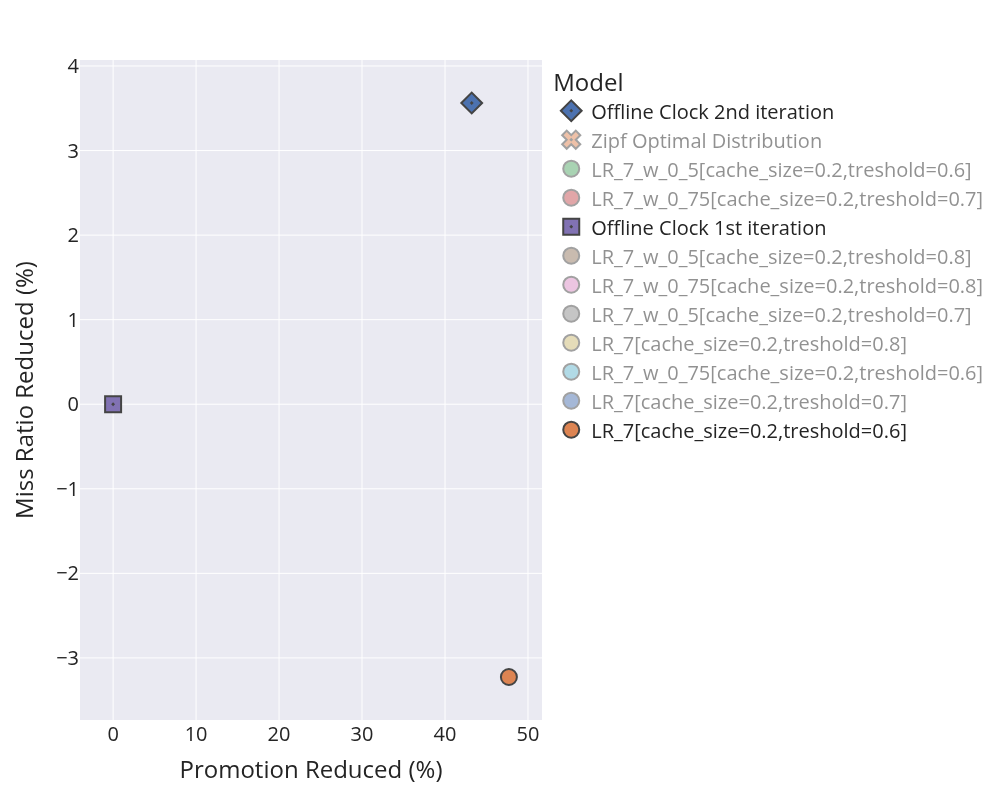
\includegraphics[width=\linewidth]{gambar/hasil/aggressive_0_2.png}
    \caption{20\% Cache Size}
    \label{fig:agg_20pct}
  \end{subfigure}
  \caption{Aggressive Model performance across cache sizes.
  Negative values indicate performance degradation and thrashing.}
  \label{fig:agg_grid}
\end{figure*}

\subsubsection{Configuration B: Aggressive Model (Unweighted Loss)}
The Aggressive Model was trained without class balancing. As
predicted by the class imbalance problem
\cite{Cunningham2008Supervised}, the model converged to a local
minimum by predicting the majority class ("Wasted") too frequently.

The results, shown in Figures \ref{fig:agg_1pct} through
\ref{fig:agg_20pct}, demonstrate a systemic failure of this strategy:
\begin{itemize}
  \item \textbf{Service Degradation:} A spike in Miss Ratio (negative
    values on the Y-axis graphs) of approximately 2\% was observed
    compared to Standard CLOCK.
  \item \textbf{Cache Thrashing:} The model aggressively evicted
    useful content, causing the cache to reload data frequently from
    the backend, increasing latency.
\end{itemize}

\subsubsection{Summary of Tuning Results}
The comparison between Conservative and Aggressive models confirms
that for latency-sensitive applications (such as CDNs or databases),
the **Conservative Model** is the only rational choice. The cost of a
cache miss (latency penalty) far outweighs the marginal savings in
write operations offered by the Aggressive model. Consequently, the
Conservative configuration was selected as the final
\textbf{PredCLOCK} implementation for the comparative analysis in
Table \ref{tab:comparison_all}.
